\section{Мета роботи}
Освоєння аналітичних методів аналізу трудомісткості
обчислювальних алгоритмів.

\section{Хід роботи}
1) З табл. 1.2 обрати логічну схему алгоритму (ЛСА) відповідно до
варіанта.
\begin{figure}[h]
    \centering
    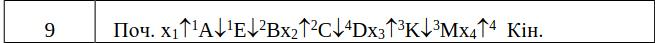
\includegraphics[width=16cm]{reports/algos/lab1/assets/1.png}
\end{figure}

З табл. 1.3 вибрати ймовірності переходів при одиничних логічних
умовах.
\begin{figure}[h]
    \centering
    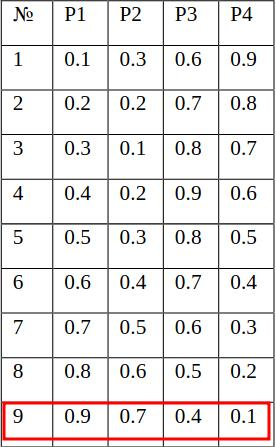
\includegraphics[width=8cm]{reports/algos/lab1/assets/2.png}
\end{figure}


\clearpage
2) За ЛСА побудувати графічну схему алгоритму, граф алгоритму та
мінімальний граф алгоритму.
\begin{figure}[h]
    \vspace{20mm} 
    \centering
    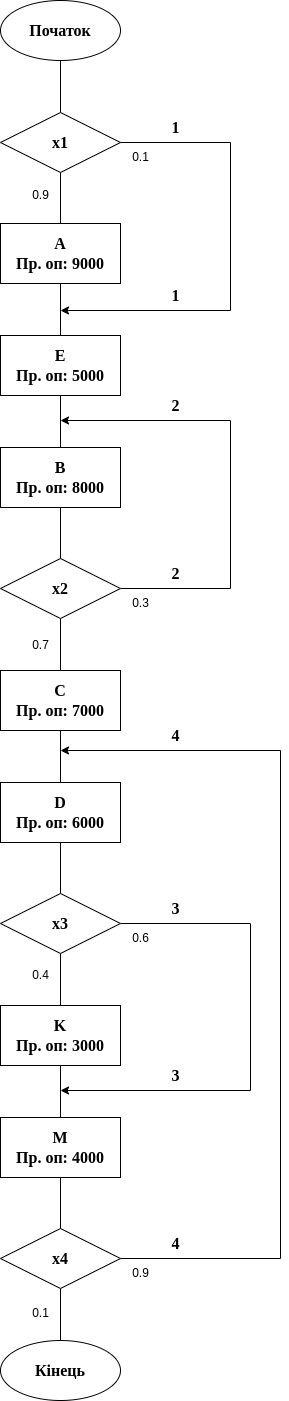
\includegraphics[width=0.2\textwidth]{reports/algos/lab1/assets/3.jpg}
    \caption{графічна схема}
\end{figure}

\begin{figure}[h]
    \centering
    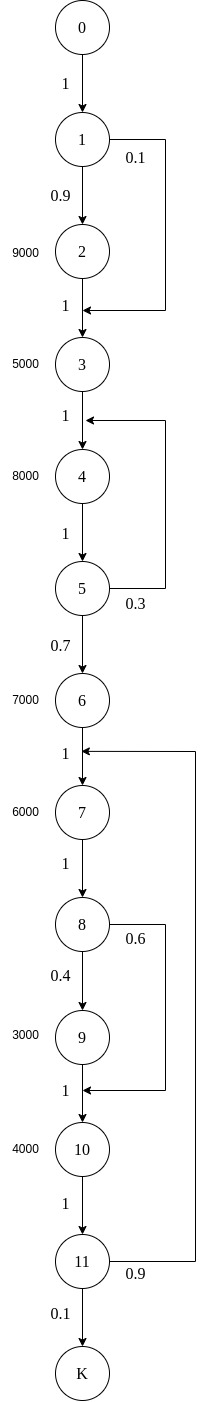
\includegraphics[width=0.2\textwidth]{reports/algos/lab1/assets/4.jpg}
    \caption{граф алгоритму}
\end{figure}

\begin{figure}[h]
    \centering
    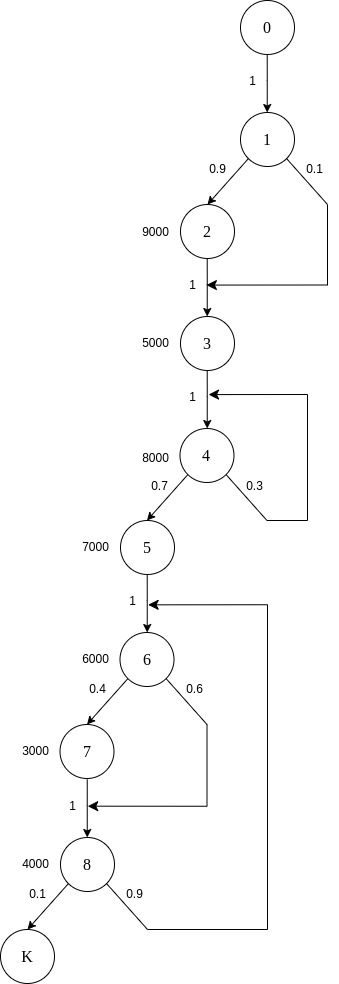
\includegraphics[width=8cm]{reports/algos/lab1/assets/5.jpg}
    \caption{мінімальний граф алгоритму}
\end{figure}

\clearpage
3) Визначити трудомісткість алгоритму методами теорії марковських
ланцюгів.
\begin{figure}[h]
    \vspace{10mm} 
    \centering
    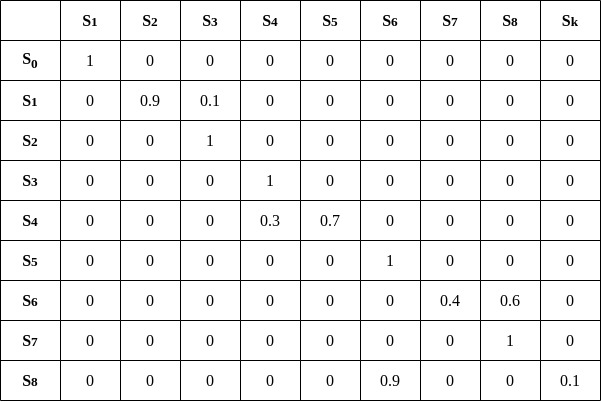
\includegraphics[width=14cm]{reports/algos/lab1/assets/6.jpg}
    \caption{Стохастична матриця алгоритму}
\end{figure}

\begin{figure}[h] 
    \centering
    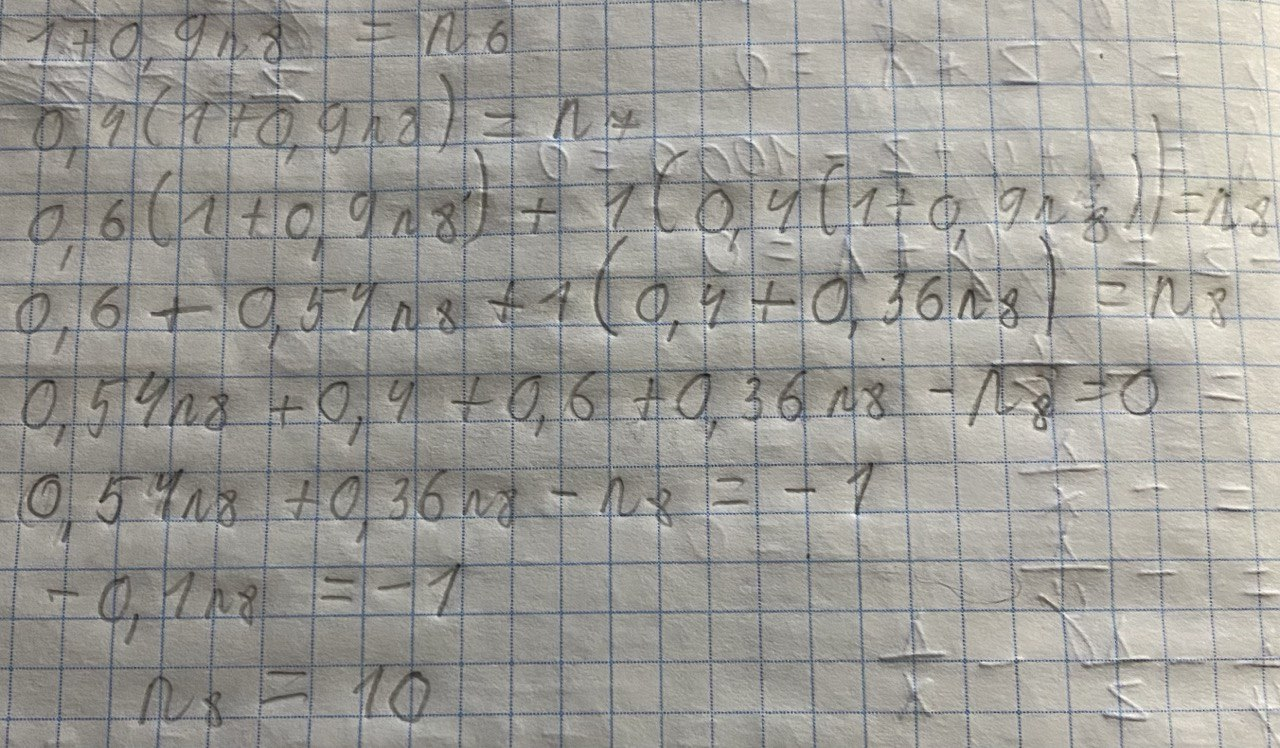
\includegraphics[width=11cm]{reports/algos/lab1/assets/8.jpg}
    \caption{Обчислення кількості звертань до усіх вершин графа}
\end{figure}

\begin{figure}[h]
    \centering
    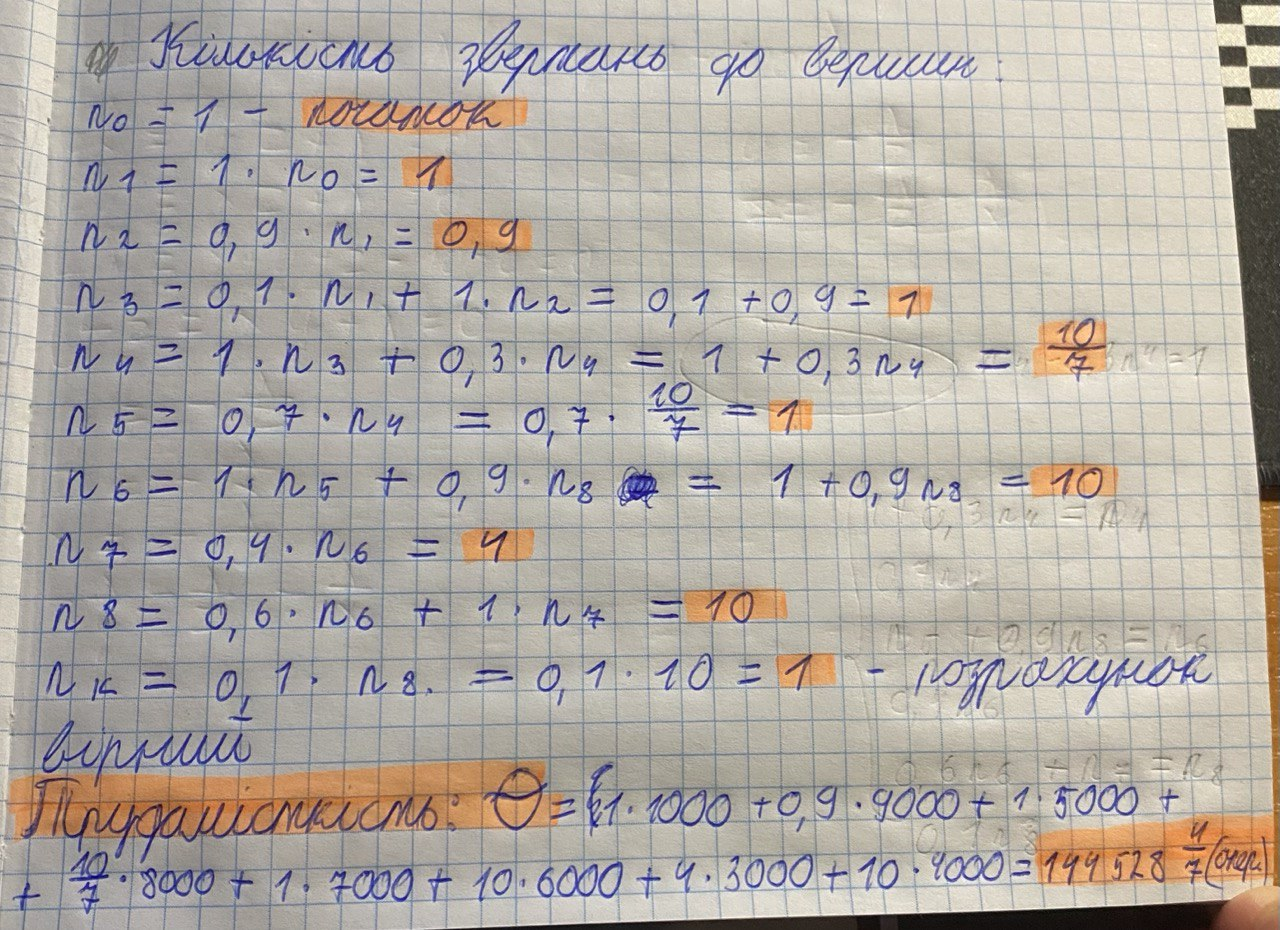
\includegraphics[width=16cm]{reports/algos/lab1/assets/7.jpg}
    \caption{Обчислення кількості звертань до усіх вершин графа та його трудомісткості}
\end{figure}

\clearpage
\section{Висновки}